\section{Opgave 1}

\begin{frame}{a) Transformationskurven}
  \begin{figure}
  \centering
      \includegraphics<1>[width=0.8\textwidth]{img/clean}
      \includegraphics<2>[width=0.8\textwidth]{img/step1}
      \includegraphics<3>[width=0.8\textwidth]{img/step2}
\end{figure}

\only<1>{Transformationskurven knytter de mulige produktionsniveauer af forskellige varer sammen.}

\only<2>{
Alle er ansat i brødindustrien $\rightarrow$ dem der er dygtigst til at bygge biler skifter branche $\rightarrow$ Bilproduktionen stiger meget, mens brødproduktionen kun falder lidt.
}

\only<3>{
Nu arbejder næsten alle i bilindustrien $\rightarrow$ de dygtigste bagere forlader branchen.
}
\end{frame}


% ------------------------------------------------------------------------------
% ------ FRAME -----------------------------------------------------------------
% ------------------------------------------------------------------------------
\begin{frame}{b) Influenza blandt de ansatte}
Landet rammes af en voldsom influenzaepidemi, hvad sker der?

\begin{itemize}
\item Influenza $\approx$ reduceret arbejdsstyrke
\item Der er både færre arbejdere til at producere brød og biler
\item Hele kurven rykker nedad
\only<2> {
\item (Hvor meget rykker den ned?)
}
\end{itemize}

\end{frame}

\begin{frame}{c) Ny brødblandingsmaskine}

    \begin{figure}
    \centering
        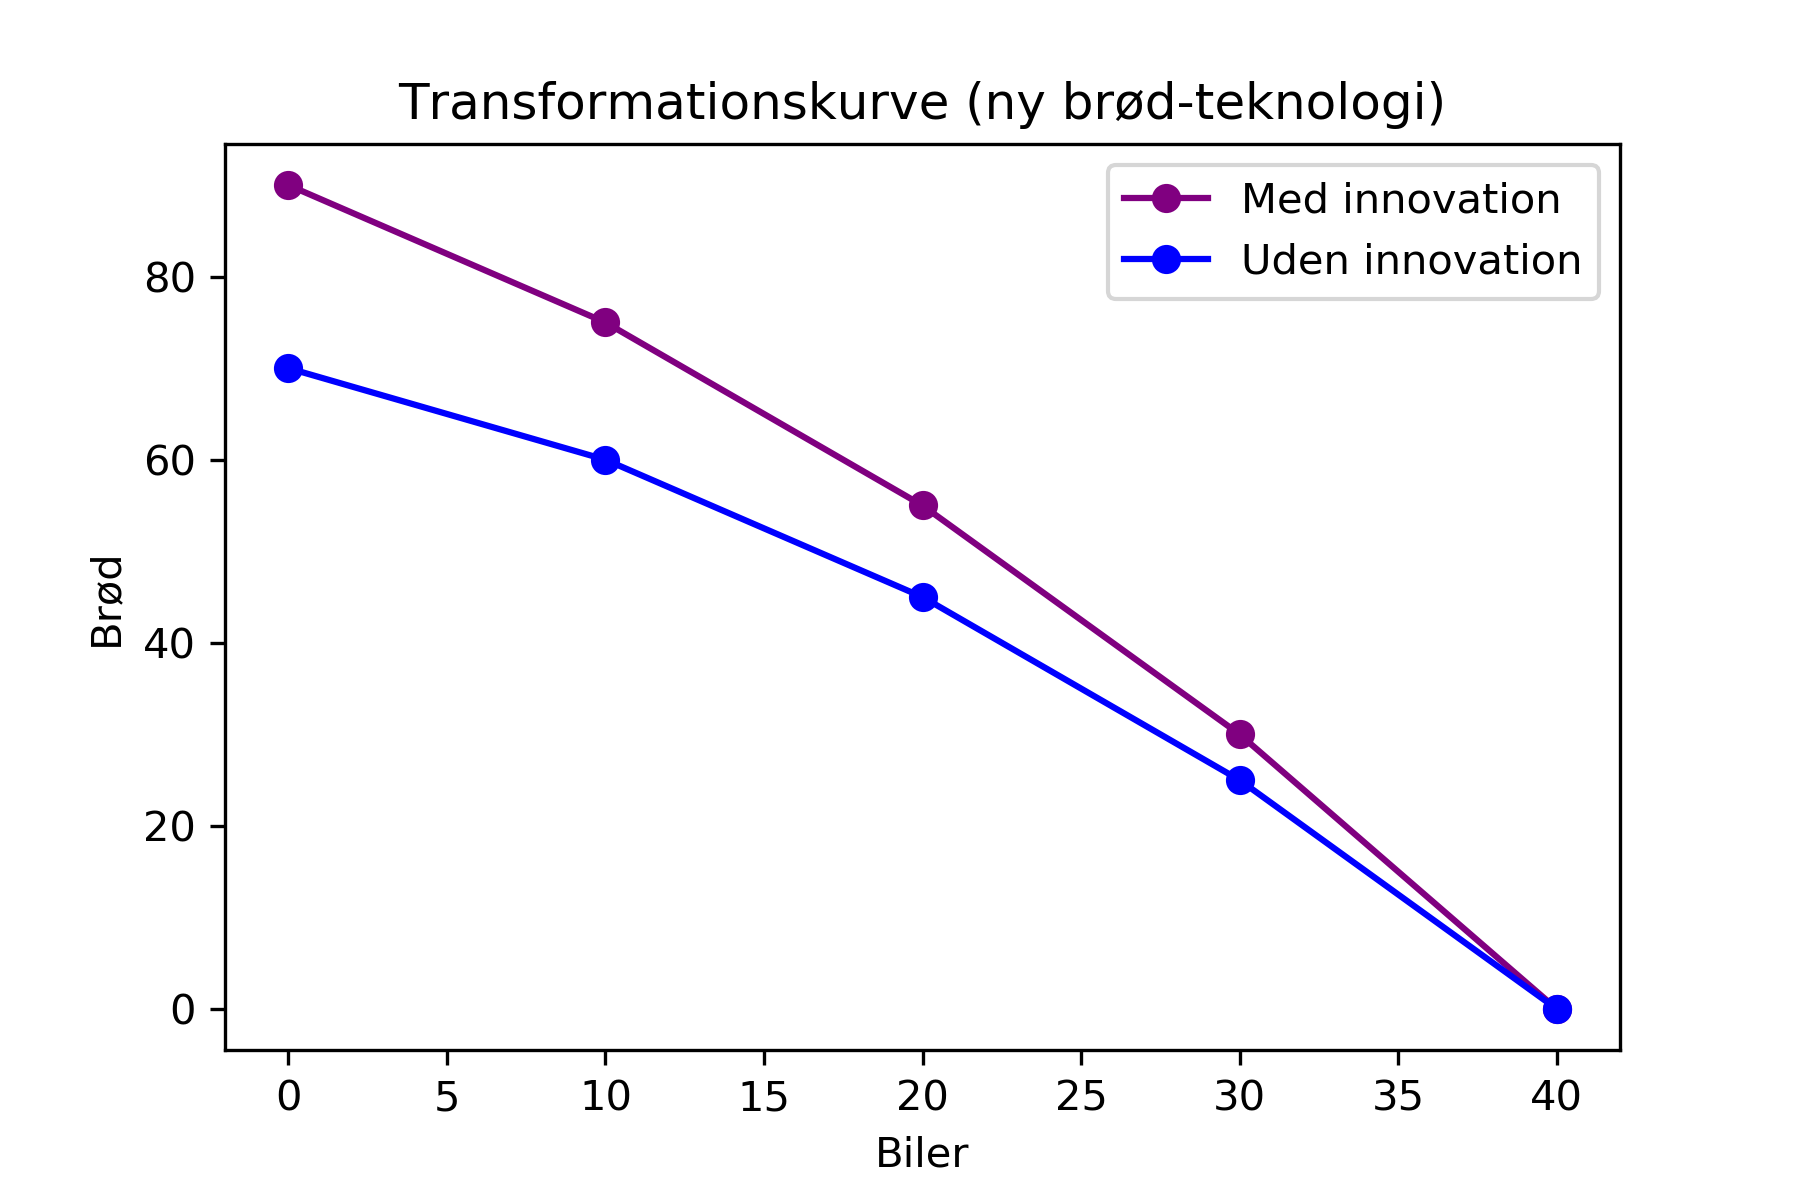
\includegraphics[width=0.8\textwidth]{img/innov}
  \end{figure}

Maskinen øger produktionen hos hver enkelt bager $\rightarrow$ mange ansatte giver stor samlet produktionsstigning.

\end{frame}


\begin{frame}{d) Arbejdsløshed}

    \begin{figure}
    \centering
        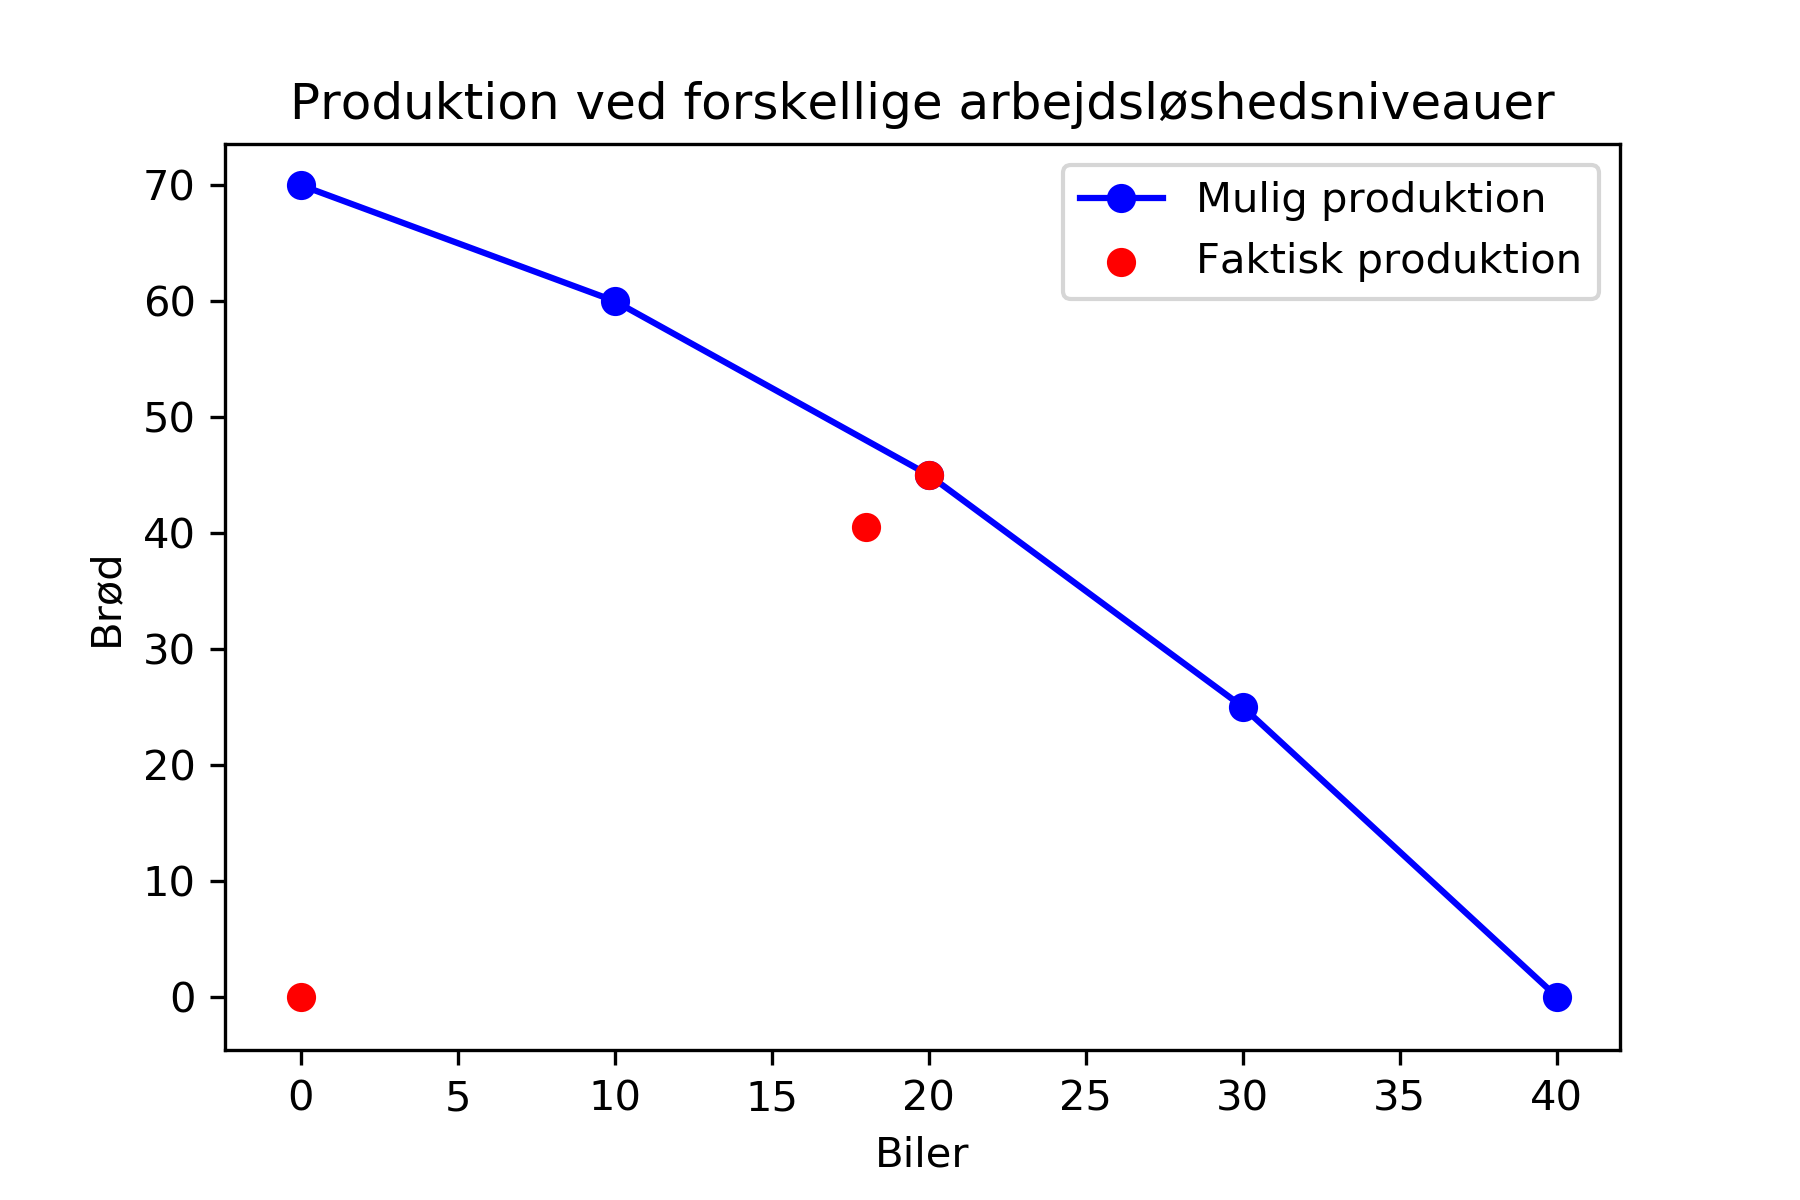
\includegraphics[width=0.8\textwidth]{img/unemp}
  \end{figure}

  \begin{itemize}
      \item[0\%] Fuld udnyttelse af potentialet i økonomien
      \item[10\%] Produktionen ligger lidt under transformationskurven
      \item[100\%] Ingen arbejder $\rightarrow$ ingen produktion $(x_1,x_2) = (0,0)$
  \end{itemize}

\end{frame}
